\documentclass[conference]{IEEEtran}
\IEEEoverridecommandlockouts
\usepackage{cite}
\usepackage{amsmath,amssymb,amsfonts}
\usepackage{graphicx}
\usepackage{textcomp}
\usepackage{xcolor}
\usepackage{url}
\def\BibTeX{{\rm B\kern-.05em{\sc i\kern-.025em b}\kern-.08em
    T\kern-.1667em\lower.7ex\hbox{E}\kern-.125emX}}

\title{A Soft Actor-Critic Method for Local Convergence Enhancement Under Strict Position--Orientation Constraints}

\author{\IEEEauthorblockN{Ze Cui}
\IEEEauthorblockA{\textit{School of Mechatronic Engineering and Automation}\\
\textit{Shanghai University}\\
Shanghai 200444, China\\
e-mail: cuize0421@126.com}
\and
\IEEEauthorblockN{Xuefeng Ji}
\IEEEauthorblockA{\textit{School of Mechatronic Engineering and Automation}\\
\textit{Shanghai University}\\
Shanghai 200444, China\\
e-mail: 15157376112@163.com}
\and
\IEEEauthorblockN{Jiaxiang Han}
\IEEEauthorblockA{\textit{School of Mechatronic Engineering and Automation}\\
\textit{Shanghai University}\\
Shanghai 200444, China\\
e-mail: 13403858438@163.com}
\and
\IEEEauthorblockN{Hai Huang}
\IEEEauthorblockA{\textit{School of Mechatronic Engineering and Automation}\\
\textit{Shanghai University}\\
Shanghai 200444, China\\
e-mail: huanghaha@shu.edu.cn}}

\begin{document}
\maketitle

\begin{abstract}
Prior work has established the feasibility of deep reinforcement learning for random end-effector pose reaching. However, as the success tolerance is tightened from the centimeter scale to the millimeter scale, policy performance may deteriorate in the target neighborhood, with position and orientation constraints becoming difficult to satisfy simultaneously and deterministic pose-holding failures emerging. This paper studies how to improve the local convergence of Soft Actor-Critic (SAC) for high-precision position--orientation control without narrowing the target distribution or introducing an analytical controller. We introduce local Jacobian features, coupled pose-precision optimization signals, and precision-boundary experience replay to form an enhanced framework. The curriculum progressively tightens position and orientation tolerances, and multi-seed deterministic evaluation is used as the promotion criterion. Under a unified random target distribution, network architecture, precision curriculum, and fixed training budget, the proposed method achieves a success rate of 96.35\% at a position--orientation tolerance of 10 millimeters and 0.10 radians, and further reaches a strict tolerance of 1 millimeter and 0.025 radians, where deterministic evaluation attains a success rate of 97.20\%.
\end{abstract}

\begin{IEEEkeywords}
reinforcement learning, soft actor-critic, robotic manipulation, position--orientation control, curriculum learning, local convergence
\end{IEEEkeywords}

% Place the main method figure early so it appears at the top of page 2,
% before the detailed method and equation blocks.
\begin{figure*}[htbp]
\centering
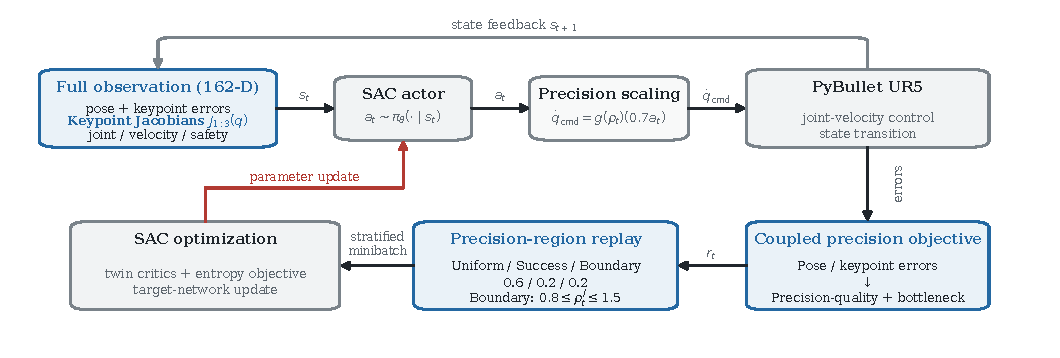
\includegraphics[width=0.92\textwidth]{figures/fig1_framework.pdf}
\caption{Learning loop of Full. Keypoint Jacobians augment the actor observation, coupled pose signals form the reward, and uniform, success, and boundary subsets feed SAC optimization. Red arrows denote parameter updates.}
\label{fig:framework}
\end{figure*}

\section{Introduction}
Random six-dimensional end-effector pose reaching requires a policy to handle three-dimensional position and three-dimensional orientation simultaneously. SAC improves exploration efficiency in continuous control through a maximum-entropy objective \cite{haarnoja2018sac}, while curriculum learning can organize training from easier tasks to progressively tighter target tolerances \cite{bengio2009curriculum}. However, they do not guarantee corrective actions with appropriate direction and magnitude near the target, which is necessary for satisfying strict position--orientation constraints.

Existing studies have reported the feasibility of reinforcement learning for random pose control. For example, MAPPO-IK obtained millimeter-level position errors and small orientation errors on random position and orientation tasks \cite{zhao2024mappoik}; continuous pose representations have also been combined with experience replay and curriculum learning to improve training convergence \cite{hu2025rtpc}. However, many random pose reaching studies mainly report final success rates or terminal errors, leaving the local performance degradation caused by continuously tightening success tolerances insufficiently analyzed.

This paper asks how local convergence degradation in high-precision position--orientation control can be reduced while keeping the target distribution, action space, and training budget fixed. We construct an enhanced framework around local kinematic guidance, coupled error optimization, and precision-region experience coverage, and analyze its performance through baseline comparison and component ablation.

The main contributions are as follows:
\begin{itemize}
  \item We study performance degradation as SAC transitions from global reaching to fine convergence in the target neighborhood under strict position--orientation tolerances, and establish a fixed-budget, multi-stage precision curriculum with deterministic evaluation.
  \item Based on an existing keypoint representation of end-effector pose, we introduce Keypoint Jacobian local kinematic information, coupled pose-precision optimization signals, and precision-boundary experience resampling to construct an enhanced SAC framework.
  \item We evaluate local convergence at different precision stages through baseline comparisons and ablations under a unified training budget.
\end{itemize}

\section{Related Work}
\subsection{Continuous Control and Curriculum Learning}
SAC balances exploration and return through a maximum-entropy objective \cite{haarnoja2018sac}. Curriculum learning organizes tasks from easy to difficult and can improve the learnability of challenging tasks \cite{bengio2009curriculum}; automated curricula for accurate motion planning likewise show the benefit of organizing training by task complexity \cite{cho2025autocurriculum}. In robotic manipulation, these mechanisms alleviate exploration over broad task ranges but do not directly ensure fine corrective actions near a pose target.

\subsection{Pose Representation and Experience Replay}
Pose representation affects error continuity and policy gradients. Continuous pose representations combined with replay and curriculum can improve convergence \cite{hu2025rtpc}, while HER and PER alter experience reuse through goal relabeling or nonuniform sampling \cite{andrychowicz2017her,schaul2016sac}. Portela \emph{et al.} encode pose with three end-effector-aligned keypoints \cite{portela2025wholebody}; observation--action alignment studies further motivate matching the representation to the control interface and reward structure \cite{bhat2026alignment}. We extend the keypoint representation with local Jacobian information for strict local convergence.

Multiple objectives in a complex reward can compete as position and orientation tolerances tighten. Reward curricula and nonlinear fusion have been studied to coordinate such objectives \cite{freitag2025complexreward,jiang2025rfm}. Clustering replay and distribution-aware sampling likewise demonstrate the value of selective sampling for state coverage and distribution preservation \cite{li2022clusteringreplay,garg2026distributionreplay}. Our replay design specifically targets the coupled precision boundary rather than assigning priority from a generic transition score.

\section{Problem Definition}
Consider a six-degree-of-freedom robotic manipulator. At time $t$, the joint state is $q_t$, the policy outputs a joint-velocity action $a_t=\dot q_t$, the end-effector pose is $T(q_t)=[R(q_t),p(q_t)]$, and the target pose is $T_g=[R_g,p_g]$. The position and orientation errors are
\begin{equation}
e_p=\|p(q_t)-p_g\|_2,
\qquad
e_R=\|\log(R_g^{\mathsf T}R(q_t))\|_2 .
\label{eq:pose_error}
\end{equation}
Given position and orientation thresholds $\epsilon_p^l$ and $\epsilon_R^l$, define the worst normalized constraint as
\begin{equation}
\rho_t^l=\max\left(\frac{e_{p,t}}{\epsilon_p^l},\frac{e_{R,t}}{\epsilon_R^l}\right).
\label{eq:rho}
\end{equation}
Let $h_t$ denote the success-hold counter. When the position and orientation thresholds are continuously satisfied for $H=5$ control steps, the success event at level $l$ is defined as
\begin{equation}
\mathcal{S}_l=\mathbb{I}[\rho_t^l\leq1\;\wedge\;h_t\geq H].
\label{eq:success}
\end{equation}
The training objective is to maximize $\Pr(\mathcal{S}_l=1)$ over the complete random target distribution.

\section{Method}
\subsection{Overall Framework and Base Representation}
KP-SAC-Base combines explicit pose errors, the three-keypoint representation of Portela \emph{et al.}, keypoint-distance and progress rewards, and uniform replay. Under the same target distribution, network architecture, SAC settings, curriculum, and budget, Full adds Keypoint Jacobians, coupled precision signals, and precision-boundary replay (Fig.~\ref{fig:framework}). M1, M2, and M3 remove bottleneck shaping, Boundary Replay, and Jacobian input, respectively, while preserving the remaining Full configuration.

\subsection{Keypoints and Local Kinematic Input}
Our keypoint construction follows the keypoint pose representation of Portela \emph{et al.} \cite{portela2025wholebody}. A cube centered at the end-effector position and rotated with the end-effector orientation is constructed in the end-effector frame, and three vertices with direct correspondence are selected. Three non-collinear points with fixed correspondence jointly encode end-effector translation and rotation. Compared with directly concatenating Euler angles or quaternions, this geometric representation converts the position--orientation error into point errors in a common coordinate space. For the fixed-base UR5 considered here, the cube has an edge length of $0.5$ m; this is a virtual geometric scale for pose encoding rather than the physical tool size. The offsets of the three vertices in the tool frame are
\begin{equation*}
\begin{aligned}
u_1&=\tfrac{0.5}{2}[1,1,1]^{\mathsf T}, &
u_2&=\tfrac{0.5}{2}[1,-1,-1]^{\mathsf T},\\
u_3&=\tfrac{0.5}{2}[-1,1,-1]^{\mathsf T}.&&
\end{aligned}
\end{equation*}
The target and current keypoints are obtained by rotating these offsets with the corresponding pose and then translating them. Let $x_i(q)$ denote the selected current keypoint coordinates and $x_i^g$ the target keypoints. The keypoint distance is
\begin{equation}
d_k=\frac{1}{K}\sum_{i=1}^{K}\|x_i(q)-x_i^g\|_2 .
\label{eq:keypoint}
\end{equation}
For each keypoint, the local velocity satisfies $\dot x_i=J_i(q)\dot q$, where $J_i\in\mathbb{R}^{3\times6}$ is the keypoint Jacobian. Recent Jacobian-exploratory reinforcement learning work also uses local Jacobian features to augment the state representation \cite{tian2025jedprl}. Full concatenates normalized keypoint errors, keypoint progress, and local Jacobian information with the standard pose errors as the policy input. Specifically, keypoint errors are divided by $0.65$ m and clipped to $[-1,1]$, while each $J_i$ is divided by $1.1$ and clipped to $[-1,1]$; the three $J_i$ are concatenated into $9\times6=54$ dimensions. The Base observation has 108 dimensions and the Full observation has 162 dimensions. To keep network capacity consistent, M3 retains the same input dimension and sets the corresponding 54 Jacobian features to zero. The observation also contains normalized joint positions and velocities, explicit position/orientation errors, end-effector velocity, and safety-related features. The Jacobian is computed from the UR5 kinematic model and the current joint state and is provided as a policy observation.

\subsection{Joint Optimization Signals}
With $\Delta e_p=e_{p,t-1}-e_{p,t}$ and $\Delta e_R=e_{R,t-1}-e_{R,t}$, the reward is summarized as
\begin{equation}
r_t=r_{\mathrm{task}}+\lambda_p\Delta e_p+\lambda_R\Delta e_R
 +\lambda_k\Delta d_k-r_{\mathrm{cost}} .
\label{eq:reward}
\end{equation}
Here, $r_{\mathrm{task}}$ is the coupled success reward and $r_{\mathrm{cost}}$ covers action and collision costs. Base retains keypoint tracking, keypoint progress, continuous success rewards, and the action and collision costs. Full and M1--M3 additionally use level-normalized precision-quality and hold/leave terms. With $\rho_p=e_p/\epsilon_p^l$ and $\rho_R=e_R/\epsilon_R^l$,
\begin{equation}
q_{\mathrm{pq}}=\exp\left[-\frac{\rho_p/0.05+\rho_R/0.10}{2}\right],
\end{equation}
where $0.05$ and $0.10$ are fixed empirical scales. Full further applies nonterminal bottleneck shaping to the worst normalized constraint:
\begin{align}
\rho_b(s_t)&=\max\left(\frac{e_{p,t}}{\epsilon_p^l},\frac{e_{R,t}}{\epsilon_R^l}\right),\\
\Phi_b(s_t)&=5\exp[-\rho_b(s_t)/2],\\
r_{b,t}&=(1-d_t)[\gamma\Phi_b(s_{t+1})-\Phi_b(s_t)].
\label{eq:bottleneck}
\end{align}
Here, $d_t=1$ denotes success, timeout, collision, or another hard-failure termination. Bottleneck shaping is zero on every terminal transition, while dedicated terms handle terminal outcomes; M1 removes only this potential term and retains precision quality and hold/leave. Table~\ref{tab:fullcomponents} lists the remaining definitions and fixed parameters.

\begin{table}[htbp]
\caption{Key training components of Full.}
\label{tab:fullcomponents}
\centering
\begin{tabular}{p{0.30\columnwidth}|p{0.60\columnwidth}}
\hline
Component & Formulation / setting\\
\hline
Precision-quality shaping & $q_{\mathrm{pq}}=\exp[-(\rho_p/0.05+\rho_R/0.10)/2]$, $w_{\mathrm{prog}}=2.0$\\
Precision-region retention & $r_{\mathrm{hold}}=0.15$, $r_{\mathrm{leave}}=-0.2$\\
Success replay & $\mathcal{S}_l=1$ transitions\\
Boundary replay & $0.8\leq\rho_t^l\leq1.5$\\
Replay mixture & Uniform / Success / Boundary $=0.6/0.2/0.2$\\
Bottleneck shaping & $\Phi_b=5\exp(-\rho_b/2)$\\
\hline
\end{tabular}
\end{table}

\subsection{Precision-Boundary Experience Replay}
Experience generated at loose curriculum stages does not sufficiently cover states near strict thresholds. For a transition $(s_t,a_t,r_t,s_{t+1})$, Full stores successful-episode transitions in the Success subset and uses the current-state condition $0.8\leq\rho_t^l\leq1.5$ for the Boundary subset; $s_{t+1}$ distinguishes holding, leaving, and single-component failure. The fixed mixture increases sampling of state--action pairs near the coupled precision boundary without replacing the uniform replay stream. M2 removes only the Boundary component.

\subsection{Automatic Precision Curriculum}
Fig.~\ref{fig:curriculum} shows the shared curriculum. Let $\rho_t=\max(e_{p,t}/\epsilon_p,e_{R,t}/\epsilon_R)$. We use $g(\rho_t)=0.05+0.05\rho_t$ for $\rho_t\leq1$ and $0.10+0.90\min(\rho_t-1,1)^2$ otherwise, with $\dot q_{\rm cmd}=g(\rho_t)(0.7a_t)$. After at least $50{,}000$ transitions per level, a deterministic probe runs every $300{,}000$ transitions using three seeds and 300 episodes each. Promotion requires aggregate/seed success of $0.85/0.80$, collision/timeout rates below $0.10/0.05$, every task-space bin above $0.60$, and a subsequent 1000-episode-per-seed confirmation under the same criterion. Online stochastic-policy success is retained only as a training diagnostic.

\begin{figure}[htbp]
\centering
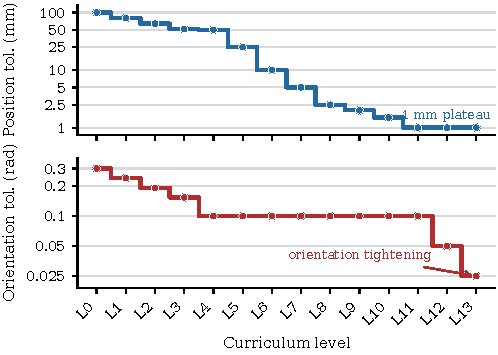
\includegraphics[width=\columnwidth]{figures/fig_curriculum_schedule.pdf}
\caption{Position and orientation tolerances across curriculum levels. Position tolerance reaches a 1-mm plateau at $L11$, after which orientation tolerance is tightened from $0.10$ to $0.025$ rad.}
\label{fig:curriculum}
\end{figure}

\section{Experimental Setup}
\subsection{Environment and Training}
IK is used only for offline target-reachability filtering and does not generate policy actions. Experiments are conducted in an obstacle-free PyBullet UR5 environment. Target positions are sampled from the initial end-effector position by first sampling $d\sim U(0.03,0.50)$ m and a uniformly distributed direction on the unit sphere, followed by $p_g=p_0+d\,v$. The target orientation difference is sampled as $\theta\sim U(0.03,\pi)$; the rotation axis is obtained by normalizing a three-dimensional standard Gaussian vector, and the axis-angle increment is composed with the initial orientation. Candidate targets are filtered for workspace validity, IK reachability, and self-collision. The filtered target distribution is shared across precision levels and methods. Each episode runs for at most 500 control steps, with a physics step of 0.00417 s and a control period of 0.05 s. Initial joint states are sampled within joint limits and filtered for self-collision. The policy action is a joint-velocity command. All methods use the same SAC hidden-layer structure, hyperparameters, target distribution, and budget of 6,000,000 transitions. Full and KP-SAC-Base use training seeds 11001 and 11002; M1, M2, and M3 use the prespecified single training seed 11001. Final frozen evaluation uses independent test seeds 31001, 31002, and 31003. Each policy checkpoint is evaluated deterministically for 1000 episodes per combination. Fig.~\ref{fig:result_overview} summarizes the common-tolerance comparison and highest reached precision. The single-seed ablations are used to compare performance after component removal and not to estimate variance across training seeds.

The component configurations of the comparison methods are listed in Table~\ref{tab:methods}.
\begin{table}[htbp]
\caption{Ablation matrix. A check mark denotes an enabled component.}
\label{tab:methods}
\centering
\begin{tabular}{l|cccc}
\hline
Method & KP & Jac. & Coupled & Boundary\\
\hline
Base & $\checkmark$ &  &  &  \\
Full & $\checkmark$ & $\checkmark$ & $\checkmark$ & $\checkmark$\\
M1 & $\checkmark$ & $\checkmark$ &  & $\checkmark$\\
M2 & $\checkmark$ & $\checkmark$ & $\checkmark$ &  \\
M3 & $\checkmark$ &  & $\checkmark$ & $\checkmark$\\
\hline
\end{tabular}
\end{table}
M3 preserves the 162-dimensional actor input by zeroing the 54 Jacobian channels.

\subsection{Evaluation Metrics}
The main metrics are coupled pose success rate, timeout rate, collision rate, and the P95 terminal position and orientation errors. P95 is computed over all frozen-evaluation episodes, including both successful and failed episodes.

\section{Results and Analysis}
\begin{figure*}[htbp]
\centering
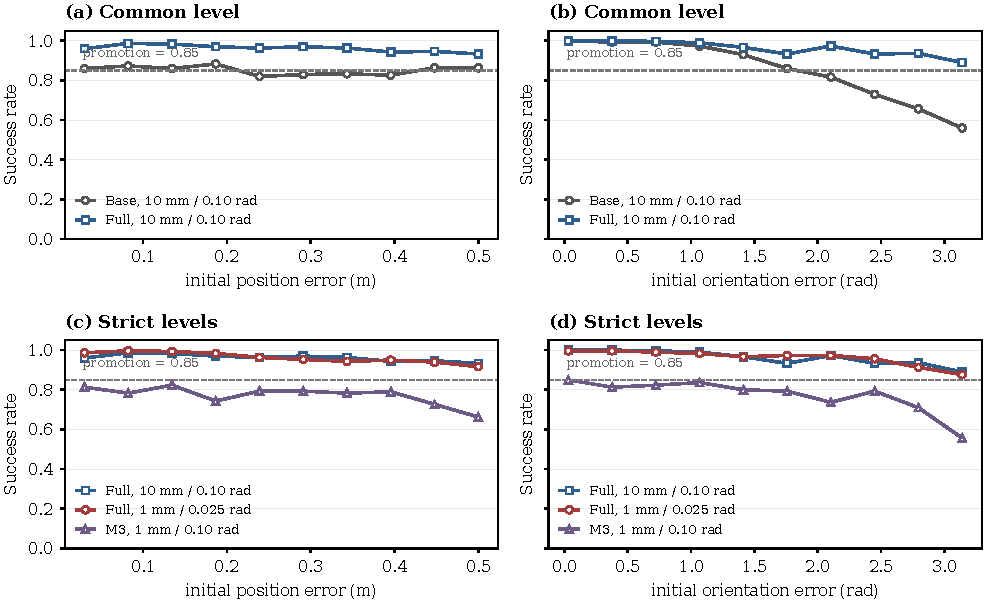
\includegraphics[width=0.92\textwidth]{figures/fig3_task_space_profiles.pdf}
\caption{Task-space success profiles under deterministic evaluation. Panels (a) and (b) show the common L6; panels (c) and (d) compare the stricter levels reached by Full and M3. The dashed line marks the 0.85 promotion criterion.}
\label{fig:profiles}
\end{figure*}

\subsection{Precision Milestones Under a Fixed Budget}
The primary evaluation concerns curriculum progression under the fixed training budget. Fig.~\ref{fig:milestones} reports when each precision milestone is first attained. Frozen evaluation covers the common L6 and each method's highest reached level, with 1000 episodes per method, test seed, and level. The common L6 supports direct comparison across all methods, whereas the highest reached level records fixed-budget progression. Full, M1, and M2 reach L13; M3 reaches L11; the two Base seeds reach L7 and L6. Results are not reported for levels a method does not reach, and all methods use the same promotion criterion.

\begin{figure}[htbp]
\centering
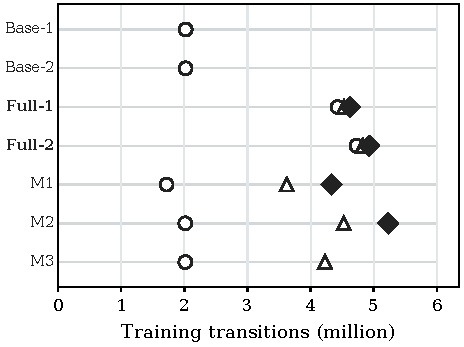
\includegraphics[width=\columnwidth]{figures/fig2_milestones.pdf}
\caption{Precision milestones within six million transitions. Circles, triangles, and diamonds denote first attainment of $10$ mm/$0.10$ rad, $1$ mm/$0.10$ rad, and $1$ mm/$0.025$ rad.}
\label{fig:milestones}
\end{figure}

\subsection{Main Results}
Fig.~\ref{fig:result_overview} combines the common-tolerance comparison with fixed-budget curriculum progression. For Full and Base, common-level statistics are computed over two training seeds and three test seeds; the ablations use one training seed and three test seeds. The key terminal P95 errors (position in millimeters / orientation in radians) are: Base at $10$ mm / $0.10$ rad: $168.85\pm7.77/0.609\pm0.040$; Full at the same tolerance: $9.31\pm0.09/0.098\pm0.000$; Full at $1$ mm / $0.025$ rad: $0.098\pm0.000/0.024\pm0.000$; M2 at the same strict tolerance: $0.99\pm0.01/0.031\pm0.002$; and M3 at $1$ mm / $0.10$ rad: $0.351\pm0.056/0.097\pm0.001$. The terminal errors of M1 are close to those of Full.

\begin{figure}[htbp]
\centering
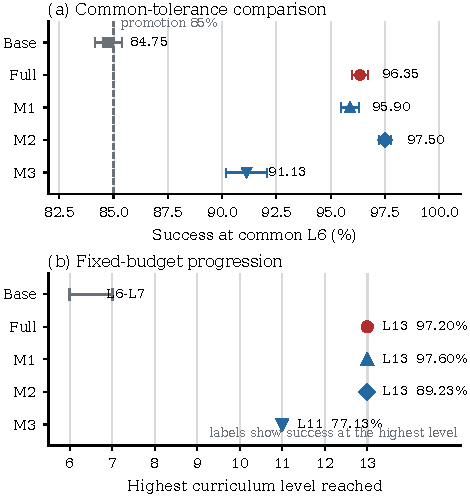
\includegraphics[width=\columnwidth]{figures/fig_result_overview.pdf}
\caption{Aggregate deterministic-evaluation results. (a) Success rate at the common $10$ mm/$0.10$ rad tolerance; error bars show standard deviation. (b) Highest curriculum level reached within six million transitions; labels report success at that level. The Base range denotes the levels reached by its two training seeds.}
\label{fig:result_overview}
\end{figure}

At the common $10$ mm / $0.10$ rad tolerance, Full increases the success rate from $84.75\%$ to $96.35\%$ and reduces terminal position P95 from $168.85$ mm to $9.31$ mm. Full also reaches $1$ mm / $0.025$ rad within the fixed training budget, whereas the two Base seeds reach only $5$ mm / $0.10$ rad and $10$ mm / $0.10$ rad. Comparisons at stricter tolerances include only methods that reach the corresponding tolerance.

Fig.~\ref{fig:profiles} further reports marginal success over the evaluation distance--orientation bins, exposing variation hidden by aggregate success rates.

At L6, Full remains between $93.3\%$ and $98.7\%$ across the initial-distance bins and between $89.0\%$ and $100\%$ across the orientation bins. The corresponding Base orientation profile decreases from $100\%$ in the smallest bin to $56.0\%$ in the largest bin. At the strict levels, Full-L13 remains above the $0.85$ promotion line in every marginal bin, whereas M3-L11 falls to $66.3\%$ in the largest distance bin and $55.7\%$ in the largest orientation bin. These profiles localize the aggregate degradation toward more difficult initial orientations and, for M3, larger initial displacements.

\subsection{Ablation Results}
M1, M2, and M3 achieve $95.90\%$, $97.50\%$, and $91.13\%$ at $10$ mm / $0.10$ rad, respectively. M3 has a larger terminal position-error P95 and progresses only to $1$ mm / $0.10$ rad. Full achieves $97.20\%$ at $1$ mm / $0.025$ rad, compared with $89.23\%$ for M2; M2 has a position-error P95 of $0.99$ mm and an orientation-error P95 of $0.031$ rad, so the degradation is concentrated in the orientation-error tail. M1 achieves $97.60\%$ at the same strict tolerance, close to Full's $97.20\%$, and no clear independent gain from Bottleneck shaping is observed in the current experiment.

\section{Discussion and Limitations}
The conclusions are limited to the obstacle-free PyBullet simulation and the specified random target distribution. The simulation does not include real encoder noise, gearbox backlash, calibration error, visual error, or communication delay. Thus, 1 mm denotes a simulated position-success tolerance and does not replace validation of real-robot accuracy. Future work should incorporate dynamic disturbances, observation noise, and real-robot experiments.

M1--M3 are targeted component ablations and use a single training seed; they therefore provide evidence of performance changes associated with component removal, not estimates of cross-seed variance or complete module-level causality. In particular, the M3 degradation is consistent with removing Jacobian information under fixed network capacity, but the evaluation does not directly measure action-direction quality or exclude other forms of local directional guidance. Similarly, M2 associates Boundary Replay removal with a larger orientation-error tail, while M1 does not establish an independent benefit from bottleneck shaping in the current setting.

\section{Conclusion}
This paper presented an SAC framework for local convergence enhancement under strict position--orientation constraints. The proposed framework raises success at $10$ mm/$0.10$ rad from KP-SAC-Base's $84.75\%$ to $96.35\%$ and reaches $1$ mm/$0.025$ rad. Without Boundary Replay, M2 achieves $89.23\%$ at this strict tolerance; without Jacobian features, M3 reaches only $1$ mm/$0.10$ rad with $77.13\%$ success. No clear independent gain from Bottleneck shaping is observed.

\begin{thebibliography}{00}
\bibitem{haarnoja2018sac} T. Haarnoja, A. Zhou, P. Abbeel, and S. Levine, ``Soft Actor-Critic: Off-Policy Maximum Entropy Deep Reinforcement Learning with a Stochastic Actor,'' in \emph{Proc. ICML}, vol. 80, pp. 1861--1870, 2018. [Online]. Available: \url{https://proceedings.mlr.press/v80/haarnoja18b.html}
\bibitem{bengio2009curriculum} Y. Bengio, J. Louradour, R. Collobert, and J. Weston, ``Curriculum learning,'' in \emph{Proc. ICML}, pp. 41--48, 2009, doi: 10.1145/1553374.1553380.
\bibitem{andrychowicz2017her} M. Andrychowicz \emph{et al.}, ``Hindsight experience replay,'' in \emph{Advances in Neural Information Processing Systems}, vol. 30, 2017. [Online]. Available: \url{https://papers.nips.cc/paper/7090-hindsight-experience-replay}
\bibitem{schaul2016sac} T. Schaul, J. Quan, I. Antonoglou, and D. Silver, ``Prioritized experience replay,'' in \emph{Proc. ICLR}, 2016. [Online]. Available: \url{https://arxiv.org/abs/1511.05952}
\bibitem{zhao2024mappoik} Y. Zhao \emph{et al.}, ``Inverse kinematics solution and control method of 6-degree-of-freedom manipulator based on deep reinforcement learning,'' \emph{Scientific Reports}, vol. 14, Art. no. 12467, 2024, doi: 10.1038/s41598-024-62948-6.
\bibitem{hu2025rtpc} Y. Hu \emph{et al.}, ``Deep reinforcement learning-based trajectory planning with continuous pose representation for 6-DoF free-floating space robot,'' \emph{Aerospace Science and Technology}, vol. 166, Art. no. 110540, 2025, doi: 10.1016/j.ast.2025.110540.
\bibitem{portela2025wholebody} T. Portela, A. Cramariuc, M. Mittal, and M. Hutter, ``Whole-Body End-Effector Pose Tracking,'' in \emph{Proc. IEEE Int. Conf. Robot. Autom. (ICRA)}, pp. 11205--11211, 2025, doi: 10.1109/ICRA55743.2025.11127964.
\bibitem{tian2025jedprl} Y. Tian, C. K. Ng, and H. Ren, ``Jacobian Exploratory Dual-Phase Reinforcement Learning for Dynamic Endoluminal Navigation of Deformable Continuum Robots,'' in \emph{Proc. IEEE/RSJ Int. Conf. Intell. Robots Syst. (IROS)}, pp. 21559--21565, 2025, doi: 10.1109/IROS60139.2025.11247575.
\bibitem{cho2025autocurriculum} D.-S. Cho, J.-M. Cho, and W.-T. Kim, ``Guided deep reinforcement learning framework using automated curriculum scheme for accurate motion planning,'' \emph{Engineering Applications of Artificial Intelligence}, vol. 139, Art. no. 109541, 2025, doi: 10.1016/j.engappai.2024.109541.
\bibitem{bhat2026alignment} V. Bhat, Z. Suleymanova, and C. Bellinger, ``Beyond Information Sufficiency: Observation-Action Space Alignment in Robotic Reinforcement Learning,'' in \emph{Proc. Canadian Conf. Artificial Intelligence}, PMLR, vol. 318, pp. 1052--1059, 2026. [Online]. Available: \url{https://proceedings.mlr.press/v318/bhat26a.html}
\bibitem{freitag2025complexreward} K. Freitag, K. Ceder, R. Laezza, K. Åkesson, and M. H. Chehreghani, ``Curriculum Reinforcement Learning for Complex Reward Functions,'' arXiv:2410.16790v2 [cs.LG], 2024. [Online]. Available: \url{https://arxiv.org/abs/2410.16790}
\bibitem{jiang2025rfm} K. Jiang, Z. Fu, J. Guo, W. Zhang, and H. Chen, ``Learning Whole-Body Loco-Manipulation for Omni-Directional Task Space Pose Tracking With a Wheeled-Quadrupedal-Manipulator,'' \emph{IEEE Robotics and Automation Letters}, vol. 10, no. 2, pp. 1481--1488, 2025, doi: 10.1109/LRA.2024.3519856.
\bibitem{li2022clusteringreplay} M. Li, T. Huang, and W. Zhu, ``Clustering experience replay for the effective exploitation in reinforcement learning,'' \emph{Pattern Recognition}, vol. 131, Art. no. 108875, 2022, doi: 10.1016/j.patcog.2022.108875.
\bibitem{garg2026distributionreplay} A. Garg, A. R. Sharma, A. Arora, and S. Verma, ``Distribution-aware sampling of replay buffer for mitigating catastrophic forgetting,'' \emph{Information Sciences}, vol. 753, Art. no. 123640, 2026, doi: 10.1016/j.ins.2026.123640.
\end{thebibliography}

\end{document}
